The InCommand component encapsulates an incoming command in a provider application. This component enforces the generic behaviour that is common to all incoming commands irrespective of their type and it provides read-only access to a command's attributes. The InCommand component is an extension of the Base Component of section \ref{sec:BaseCmp}. 

Incoming commands must be accepted before they can be executed (see section \ref{sec:CmdLifecycle}). The acceptance check is implemented partly by the InLoader (see section \ref{sec:InLoader}) and partly by the initialization and configuration checks of the InCommand itself.

The behaviour of a command that has been accepted is modelled by the state machine shown in figure \ref{fig:InCommand} (the \textit{InCommand State Machine}). This state machine is embedded within the CONFIGURED state of the Base State Machine. 

\begin{figure}[h]
 \centering
 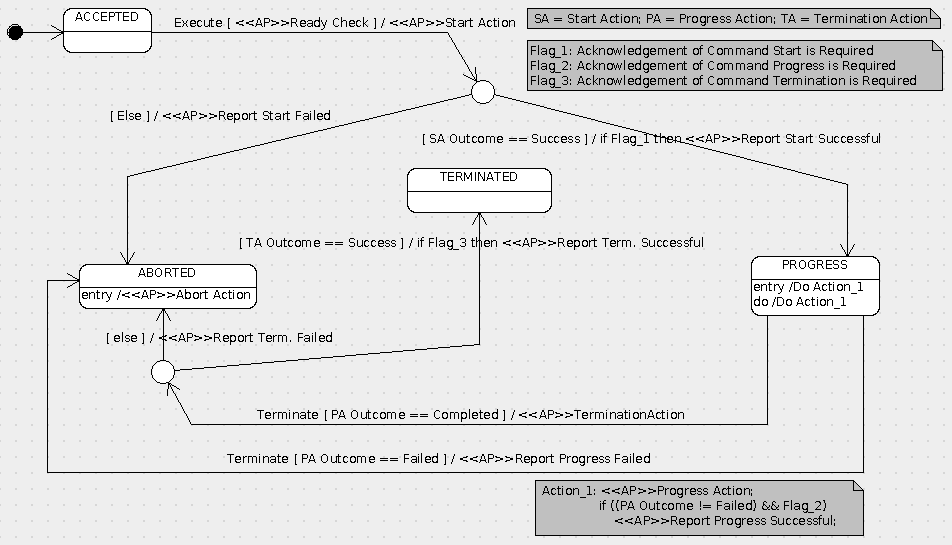
\includegraphics[scale=0.47,keepaspectratio=true]{InCommand.png}
 \caption{The InCommand State Machine}
 \label{fig:InCommand}
\end{figure}

When the state machine is started (i.e. when the command is accepted and the InCommand enters state CONFIGURED), it enters state ACCEPTED. In this state, the InCommand component waits for sequences of Execute and Terminate commands. The constraint that an InCommand component should be sent \texttt{Execute} and \texttt{Terminate} requests in sequence is enforced by the InManager which is responsible for controlling the execution of InCommands (see section \ref{sec:InManager}).

Execution of the InCommand state machine in state ACCEPTED causes it to perform the Ready Check. The Ready Check – like all other command checks and command actions – is an adaptation point.  

If the Ready Check is failed (i.e. if the Ready Check indicates that the command is not yet ready to start execution), the command remains in state ACCEPTED.

If the Ready Check is passed (i.e. if the Ready Check indicates that the command is ready to start execution), the command executes the Start Action and, depending on its outcome, it makes a transition either to state ABORTED or to state PROGRESS.  

In state PROGRESS, the command executes its Progress Action. If the completion outcome of the Progress Action is "not completed” (indicating that the command has not yet completed execution), the InCommand remains in state PROGRESS. If, instead, the completiong outcome of the Progress Action is “completed” (indicating that all progress steps have been executed), then the InCommand moves out of the PROGRESS state and executes its termination action. The outcome of the termination action determines whether the command enters TERMINATED (to indicate a nominal end of the command) or ABORTED (to indicate that either one or more of its execution steps have failed or that its termination action has failed).  

The Progress Action is responsible for updating the Progress Step Identifier. A change in the value of this identifier marks the end of a Progress Step. A Progress step is a set logically related execution steps which are executed in sequence.

If the command is neither terminated nor aborted in the first Execute-Terminate cycle, it will be sent further pairs of Execute-Terminate commands by its InManager and will repeat the behaviour described in the previous paragraphs.  

The InCommand component is responsible for generating acknowledge reports. The acknowledge reports are generated: at the end of the start action; during execution of the progress action; and at the end of the termination action. At the end of the start and termination actions, either a success or a failure acknowledge report is generated depending on the outcome of the action. During the execution of the progress action, failure reports are generated whenever an execution step fails whereas success reports are generated whenever a progress step has terminated successfully. Success reports are only generated if the corresponding acknowledge flag is set in the InCommand. 

The generation of the acknowledge reports is an adaptation point for the InCommand. Note that the acknowledge report for the command acceptance is generated by the InLoader component, see section \ref{sec:InLoader}.

The InCommand component provides visibility over all attributes of the command it \chgC{encapsulates. The operation to set and get the} value of the command attributes is therefore an adaptation point for the InCommand.

